% Section content template for individual Educative lessons
% This file contains the actual content for a specific section
% Generated from Educative API section content

% Section: Design Considerations of Yelp
% Section ID: 5518783229198336
% Section Slug: design-considerations-of-yelp
% Generated: 2025-12-07T23:22:49.557879

\subsection{Introduction}\label{rgdLlnzNCAbrCsDyRv_9g}
\\
We discussed the design, building blocks, components, and the entire workflow of our system in the previous lesson, which brought up a number of interesting questions that now need answering. For example, what approach do we use to find the places, or how do we rank places based on their popularity? This lesson addresses important design concerns like the ones we just mentioned. The table given below summarizes the goals of this lesson.

\textbf{Summary of the Lesson}

\begin{table}[htbp]
\centering
\small
\adjustbox{max width=\textwidth}{
\begin{tabular}{|p{0.289\textwidth}|p{0.661\textwidth}|}
\hline
\textbf{Section/Sub-section} & \textbf{Purpose} \\
\hline
\hline
\textbf{Searching} & This process divides the world into segments to optimize the search, so that all nearby sites in a given location and radius can be identified. \\
\hline
Storing Indexes & We index the places to improve query performance and estimate the storage required for all of the indexes. \\
\hline
Searching Using Segments & We search all the desired places by combining the segments. \\
\hline
\textbf{Dynamic Segments} & We solve the static segment limitations using dynamic segments. \\
\hline
Searching Using a QuadTree & We explore the searching functionality using a QuadTree. \\
\hline
Space Estimations for a QuadTree & We estimate the storage required for a QuadTree. \\
\hline
Data Partitioning & We look into the options we can use to partition data. \\
\hline
Ensuring Availability & We look into how we'll ensure the availability of the system. \\
\hline
Inserting a New Place & We look into how we'll insert the place in a QuadTree. \\
\hline
Ranking Popular Places & We rank the places of the system. \\
\hline
\textbf{Evaluation} & We evaluate how our system fulfills the non-functional requirements. \\
\hline
\end{tabular}
}
\caption{Summary of the Lesson}
\end{table}

\subsection{Searching}\label{OI-zEzv66pMZ-TcKFN4ZH}
\\
From Google Maps, we were able to connect segments and meet the scalability challenge to process a large graph efficiently. The graph of the world had numerous nodes and vertices, and traversing them was time-consuming. Therefore, we divided the whole world into smaller segments/subgraphs to process and query them simultaneously. The segmentation helps us improve the scalability of the system.\\
\strut \\
Each segment will be of the size \protect\phantomsection\label{katex_inline_FT89fwh1UzAhkSokzDKDz}{{{\(5 \times 5 \ \text{miles}\)}}} and will contain a list of places that exist within it. We only search a few segments to locate destinations that are close by. We can use a given location and defined radius to find all the nearby segments and identify sites that are close.

\begin{figure}[htbp]
 \centering
 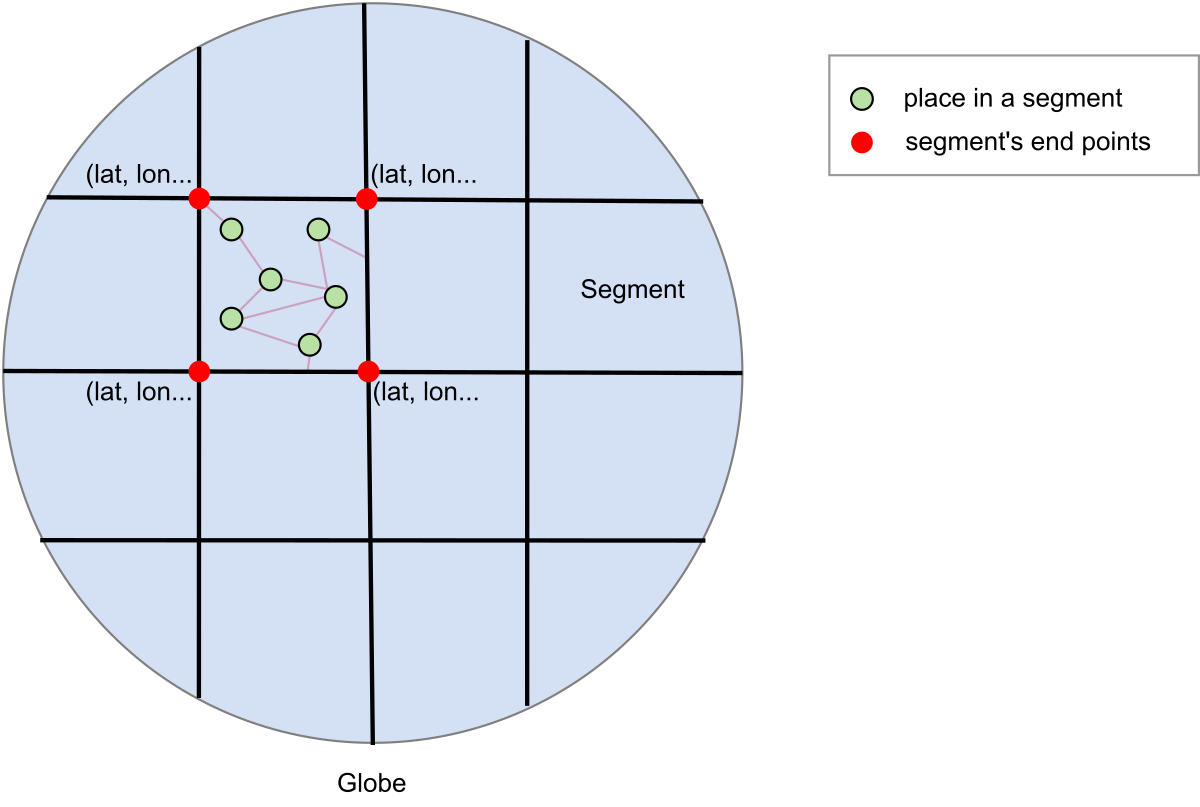
\includegraphics[width=0.5\textwidth]{Images/chapter_29/section_5518783229198336/4734340915527680.png}
 \caption{Partitioning the globe into small segments, where each segment has four coordinates (lat, long) and all segments hold the coordinates of different places}
\end{figure}

\begin{quote}
\textbf{Quiz:}
\textbf{Question 1:} How will we find nearby places if we create a table for storing all places?
\textbf{Answer:} We can make a table of places that have `Place\_ID` as a unique ID and store each place in it. The longitude and latitude columns help us specify the exact location. Indexing both of these columns can help us fetch data efficiently. We can specify each location as a pair of latitude (`M`) and longitude (`N`). We can also search for a place within a given radius of `R` by finding all the places between the latitude `M-R` and `M+R` and the longitude `N-R` and `N+R`. We can apply

Dijkstra's algorithm to find the distance between two points.
\textbf{Question 2:} How efficient will our searching be when based on the table?
\textbf{Answer:} We can have multiple lists of places within (`M-R`, `M+R`) and (`N-R`,

`N+R`). It'll be a challenge to handle concurrent requests. When queries that are used to fetch the places will be coming at a high rate for different segments, the response time and performance will be affected.
\end{quote}

We can store all the places in a table and uniquely identify a segment by having a segment\_ID. We can index each segment in the database. Now , we have limited the number of segments we need to search, so the query will be optimized and return results quickly.

\subsubsection{Improve data fetching}\label{0RnNOvxZkymu48oaJyNre}
\\
We use a key-value store for quick access to places in the segments. The key is the segment\_ID, while the \texttt{value} contains the list of places in that segment. Let 's estimate how much space we need to store the indexes.
\begin{quote}
We can usually store a few MBs in the value of the key-value store. If we assume that each segment has 500 places then it will take up \protect\phantomsection\label{katex_inline_GQkvjfaWngD3QWldDeBIz}{{{\(500 \times 1296 \ \text{Bytes = 0.648MB}\)}}}, and we can easily store it as a value.
\end{quote}
\\
The total area of the earth is around 200 million square miles, and the land surface area is about 60 million square miles. If we consider our radius to be ten miles, then we'll have 6 million segments. An 8-Byte identifier will identify each segment.
\\
Let's calculate how much memory we need.


\subsubsection{Search using segments}\label{4WSRQGmoIyhMWXU3M3nv1}
\\
A user may select a radius for searching places that aren't present in a single segment. So , we need to combine multiple segments by \href{https://www.educative.io/courses/grokking-the-system-design-interview/challenges-of-google-maps-design\#Connect-two-segments}{connecting the segments} to find locations within the specified radius---say, five miles.
\\
First, we constrain the number of segments. This reduces the graph size and makes the searching process optimizable. Then , we identify all the relevant locations, compute the distance from the searching point, and show it to the user.

\begin{figure}[htbp]
 \centering
 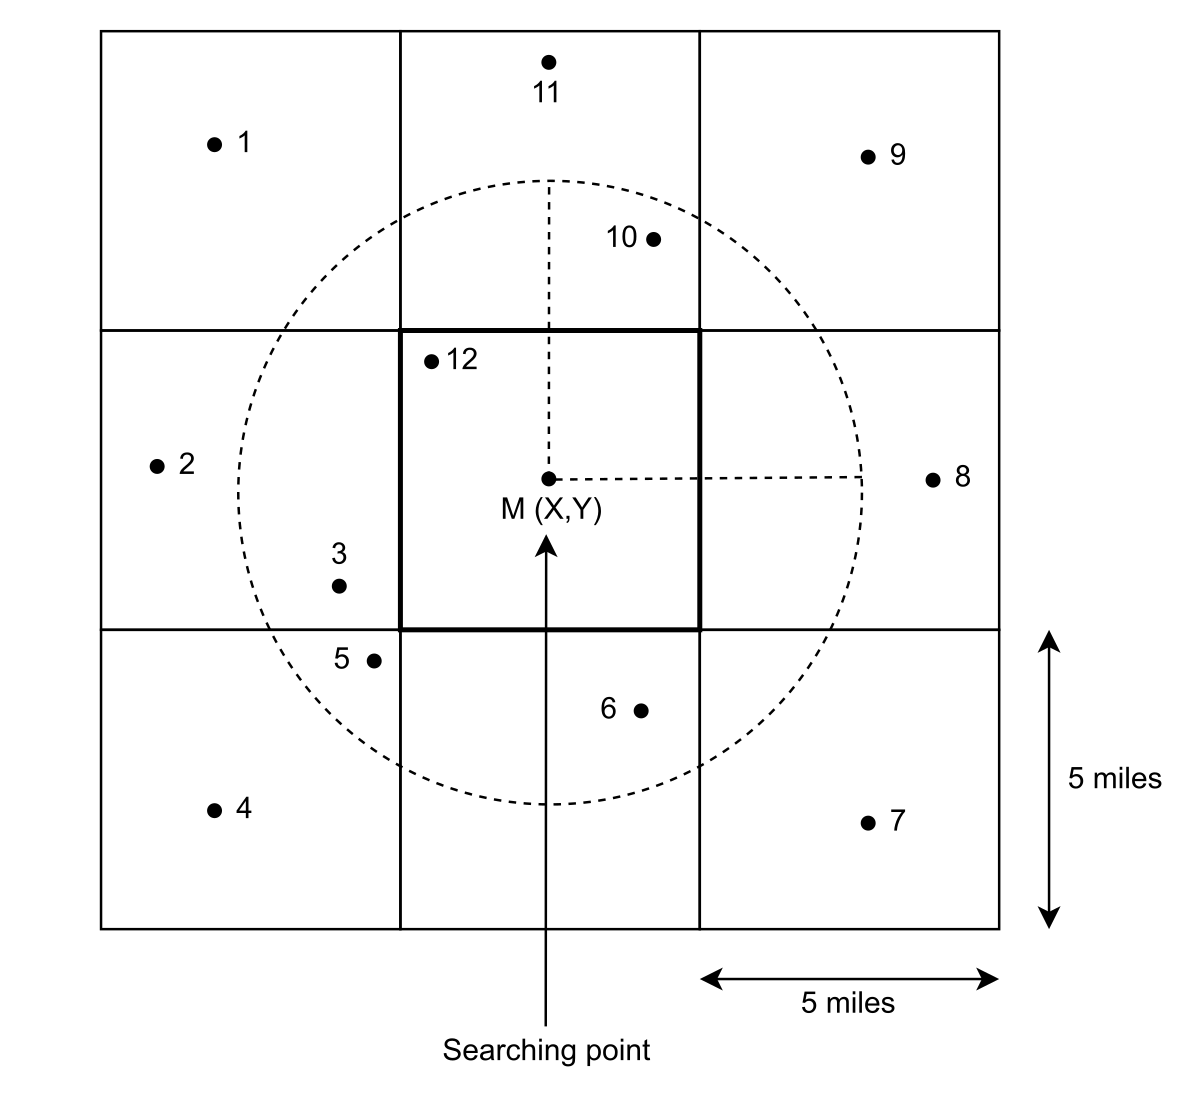
\includegraphics[width=0.5\textwidth]{Images/chapter_29/section_5518783229198336/5020776243920896.png}
 \caption{Searching for locations using segments}
\end{figure}

\begin{quote}
\textbf{Quiz:}
\textbf{Question 1:} Can you identify a problem with the current approach?
\textbf{Answer:} Our locations are not evenly distributed across segments, and this approach may still take a long time to run on segments with a lot of places. For example, in a city like New York, we can have lots of places even within a small radius because it is a densely-populated area. And for less populated areas, the same radius might not have enough places,

and we might need to expand our radius to find more.
\end{quote}

\subsection{Dynamic segments}\label{MAgF8dsxCfaJa_1VJbeNx}
\\
We solve the problem of uneven distribution of places in a segment by dynamically sizing the segments. We do this by focusing on the number of places. We split a segment into four more segments if the number of places reaches a certain limit. We assume 500 places as our limit. While using this approach, we need to decide on the following questions:

\begin{enumerate}
\item
\protect\phantomsection\label{W1GFlpFPtn6ey388ZIKFC}
How will we map the segments?
\item
\protect\phantomsection\label{DhcDu7Yc9sCzdcKFvlT-d}
How will we connect to other segments?
\end{enumerate}
\\
We use a \textbf{QuadTree}(A QuadTree is a tree data structure in which each internal node has exactly four children. QuadTrees are the two-dimensional analog of octrees and are most often used to partition a two-dimensional space by recursively subdividing it into four quadrants or regions. The data associated with a leaf cell varies by application, but the leaf cell represents a ``unit of interesting spatial information''. Source: Wikipedia) to manage our segments. Each node contains the information of a segment. If the number of places exceeds 500, then we split that segment into four more child nodes and divide the places between them. In this way, the leaf nodes will be those segments that can't be broken down any further. Each leaf node will have a list of places in it, too.

\subsubsection{Search using a QuadTree}\label{68wH-ytoe31h2b3Xv0ZQ5}
\\
We start searching from the root node and continue to visit the nodes to find our desired segment. We check every node to see if it has more child nodes. If a node has no more children, then we stop our search because that node is the required one. We also connect each child node with its neighboring nodes with a doubly-linked list. All the child nodes of all the parent nodes are connected through the doubly-linked list. This list allows us to find the neighboring segments when we can move forward and backward as per our requirement. After identifying the segments, we have the required \texttt{PlaceID} values of the places and we can search our database to find more details on them.

\begin{quote}
\textbf{Quiz:}
\textbf{Question 1:} Is there an alternative approach to find the neighboring segments?
\textbf{Answer:} We can use the pointers of parent nodes to find the neighboring segments. In each node, we can keep a pointer that points towards the parent node. Every parent node has pointers to its children nodes, so we can use those to find the adjacent leaf nodes. We can extend our search by going up through the parent pointers. In the following illustration,

node `F` can find its neighboring node, `G`, by first going to the parent node, `B`, and then to `G`.

\end{quote}

The following slides show how the process of searching for a place works. If a node has the places we need, we stop there. Otherwise, we explore more nodes until we reach our search radius. After finding the node, we query the database for information related to the places and return the desired ones.

\begin{figure}[htbp]
 \centering
 \begin{subfigure}[b]{0.48\textwidth}
 \centering
 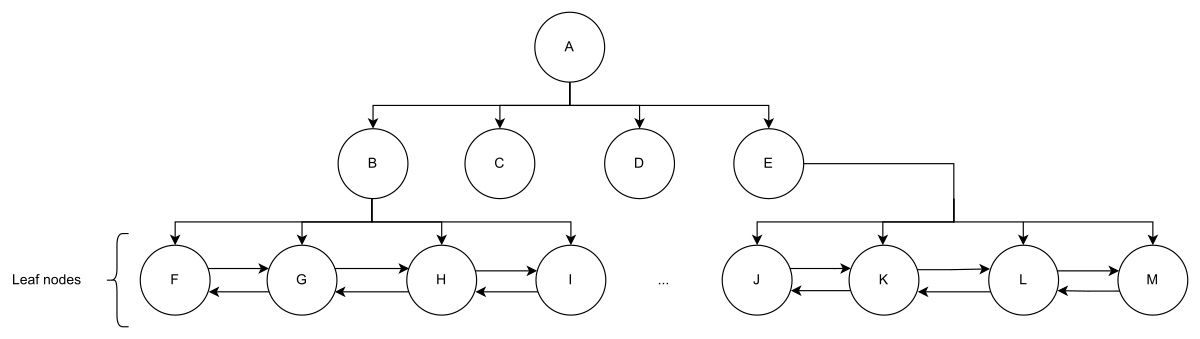
\includegraphics[width=\textwidth]{Images/chapter_29/section_5518783229198336/5116171385044992.png}
 \caption{All the leaf nodes in the QuadTree are linked, just like in a doubly-linked list}
 \end{subfigure}
 \hfill
 \begin{subfigure}[b]{0.48\textwidth}
 \centering
 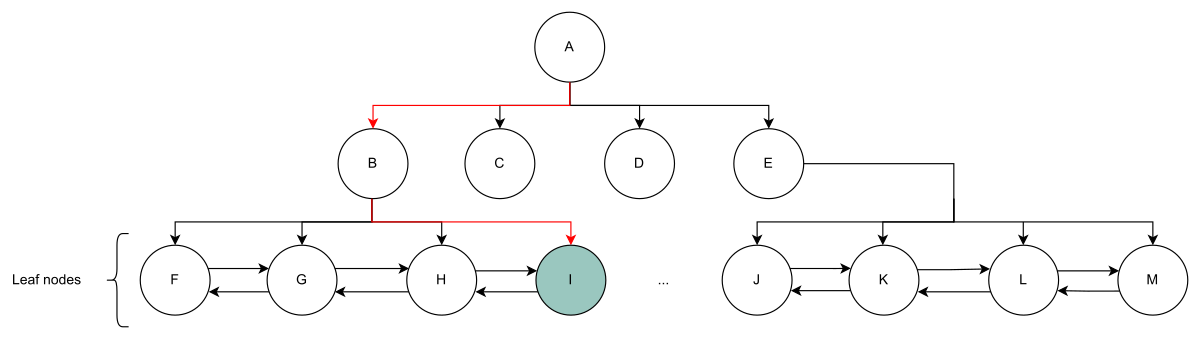
\includegraphics[width=\textwidth]{Images/chapter_29/section_5518783229198336/6160077497303040.png}
 \caption{We searched for a cafe and found the required number cafes—say, 20—in the same leaf node, so do not need to iterate any other nodes}
 \end{subfigure}
\end{figure}

\begin{figure}[htbp]
 \centering
 \begin{subfigure}[b]{0.48\textwidth}
 \centering
 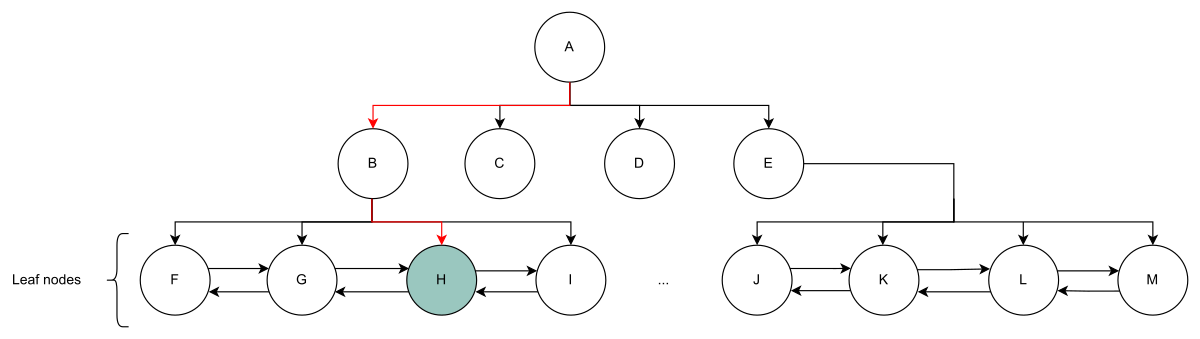
\includegraphics[width=\textwidth]{Images/chapter_29/section_5518783229198336/5338450681397248.png}
 \caption{We searched for a cafe but only found, say, six cafes in a leaf node}
 \end{subfigure}
 \hfill
 \begin{subfigure}[b]{0.48\textwidth}
 \centering
 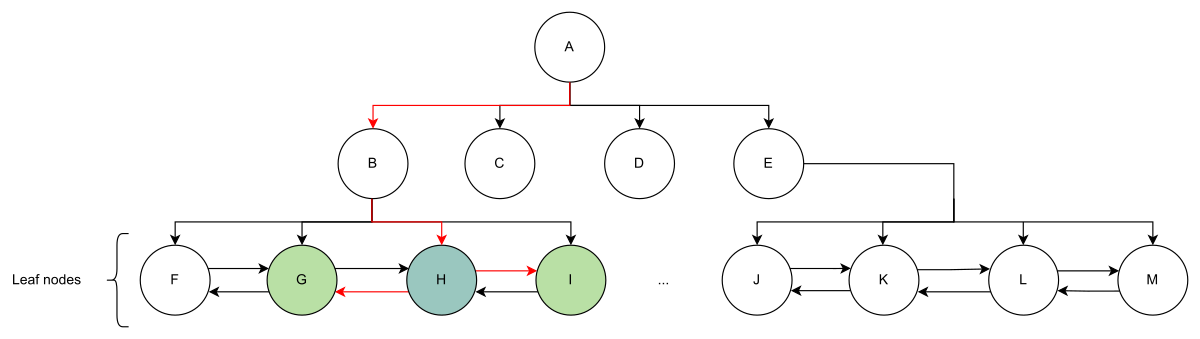
\includegraphics[width=\textwidth]{Images/chapter_29/section_5518783229198336/4944192388464640.png}
 \caption{The leaf node will explore its neighboring nodes to find more cafes}
 \end{subfigure}
\end{figure}

\subsubsection{Storage space estimation for QuadTrees}\label{ULsZmzlGE2y3ugTJqucq0}
\\
Let's calculate the storage we need for keeping QuadTrees:

\begin{itemize}
\item
\protect\phantomsection\label{u0-jBfVOI42BzTsAKzmdo}
We store the \texttt{PlaceID}, \texttt{Latitude}, and \texttt{Longitude} for each place in the node. Each of these values is of the size 8 Bytes. For 500 million places, we need the following amount of storage for all places:

\begin{itemize}
\item
\protect\phantomsection\label{katex_inline_p6foB0GuGhYpa8p-oHMwe}{{{\((8+8+8)\times10^6 \times 500 = 12 \text{GB}\)}}}
\end{itemize}
\item
\protect\phantomsection\label{mtpNteq0kVTOijSf6WCFS}
We'll have 500 places in a single node. So , for 500 million places, we'll need \protect\phantomsection\label{katex_inline__T2aWrZ-wcLwOt0nf_Xo6}{{{\(\frac{500M}{500} = 1 \text{M}\)}}} leaf nodes.
\item
\protect\phantomsection\label{S0XmhStgPkOKbZP-nI6hE}
The QuadTree with 1 million leaf nodes has approximately 1/3rd of the leaf nodes of the internal nodes(Source: https://tildesites.bowdoin.edu/\textasciitilde ltoma/teaching/cs3225-GIS/fall16/Lectures/gis\_qdt1.pdf) (all the nodes up the leaf level), and each internal node has four pointers to its child nodes. If we'll assume 8 Bytes for each pointer, then we'll need \protect\phantomsection\label{katex_inline_IVc1xn0PR2ysNU8VtbnPn}{{{\(1\text{M} \times 1/3 \times 4 \times 8 = 10.67 \text{MB}\)}}} of space for the internal nodes.
\item
\protect\phantomsection\label{iNkvYPyzxwf58AKd8dVVr}
We can get the total space needed to store all the internal nodes by adding \protect\phantomsection\label{katex_inline_GzbAQ1tP9qtfrzlwr_slg}{{{\(12\text{GB}\)}}} and \protect\phantomsection\label{katex_inline_hdNQudHhr-66AdAO-Z0C8}{{{\(10.67\text{MB}\)}}}, that is, \protect\phantomsection\label{katex_inline_vnRt_-qvBV1geOQtNqJZ6}{{{\(12.01\text{GB}\)}}} approximately.
\end{itemize}
\\
We can easily store a QuadTree on a server.
\\
Let's try the following calculator to calculate the storage needed for a QuadTree:


\subsubsection{Data partitioning}\label{lxMhyCwWsV4igX8T2BBm9}
\\
Keeping 20\% growth per year in mind, the number of places will increase. We can partition data on the following basis:

\begin{enumerate}
\item
\protect\phantomsection\label{a1XhAiNMnUoLV6EPeTCZA}
\textbf{Regions}: We can split our places into regions on the basis of zip codes. This way, all the places that belong to a specific region are stored on a single node. We store information on the region along with the place, so that we can query on the basis of regions too. We can use the user's region to find the places in that specific region. This data partitioning comes with a few challenges. For example, if a region becomes popular during tourist season, it can affect the performance of our system. We might have numerous queries on the server that might result in slow responsiveness to user queries.
\item
\protect\phantomsection\label{ckD9mA_aBG_m07wsP68eB}
\textbf{\texttt{PlaceID}}: We can partition data on the basis of \texttt{PlaceID} instead of the region to avoid the query overload in popular seasons or rush hours. We can use a key-value store to store the places. In this case, the key is the \texttt{PlaceID} and the value contains the server in which that place is stored. This will make the process of fetching places more efficient.
\end{enumerate}
\\
So, we'll opt for partitioning on the basis of places. Moreover, we'll also use caches for popular places. The cache will have information about that particular place.

\subsubsection{Ensure availability}\label{WcU2fjjhwrPDTsgpUs14c}
\\
Consider a scenario where multiple people in the same radius place a search request. If we have a single QuadTree, it'll affect the availability of the users. So, we can't rely on a single QuadTree. To cater to this problem, we replicate our QuadTrees on multiple servers to ensure availability. This allows us to distribute the read traffic and decrease the response time. Quad Trees are built on a server, so we can use the server ID as a key to identify the server on which the QuadTree is present. The value is the list of places that the QuadTree holds. The key-value store eases the rebuilding of the QuadTree in case we lose it.

\begin{quote}
\textbf{Quiz:}
\textbf{Question 1:} How will the leader-follower approach help us in replication?
\textbf{Answer:} We'll have a single leader and two followers. The leader will have the

QuadTree and it'll handle all the write requests. It'll update the followers about any change made to the QuadTrees synchronously, so there'll be a chance of delay. The followers will handle all the read requests. In case a follower dies, we'll choose another follower and replicate the data to it. If the leader is down, we`ll choose any of the followers to step in as the leader. This way, we'll be able to replicate our QuadTrees onto three servers.
\end{quote}

\subsubsection{Insert a new place}\label{40eWYU6xfphfGUdamllt3}
\\
We insert a new place into the database as well as in our QuadTree. We find the segment of the new place if the QuadTree is distributed on different servers, and then we add it to that segment. We split the segment if required and update the QuadTree accordingly.

\subsubsection{Rank popular places}\label{DvaUhNOAde9x495rYShjD}
\\
We need a service, a \textbf{rating calculator}, which calculates the overall rating of a service. We can store the rating of a place in the database and also in the QuadTree, along with the ID, latitude, and longitude of the place. The QuadTree returns the top 50 or 100 popular places within the given radius. The \textbf{aggregator service} determines the actual top places and returns them to the user.
\begin{quote}
\textbf{Note:} We don't expect the rating to be updated within hours, as such frequent changes in QuadTrees or databases can be expensive. We update them once a day, when the load is minimal.
\end{quote}
\subsection{Finalized design}\label{H43_oBw4vzcPc8RnoX8cs}
\\
We added a few new components to our design. We introduced caches to store popular places. This allows us to fetch the places much faster. Moreover , we also added a rating calculator that sorts the places based on their ratings. This will enhance user experience, since the places with a good rating will be displayed first.
\\
The updated design of our system is shown below:

\begin{figure}[htbp]
 \centering
 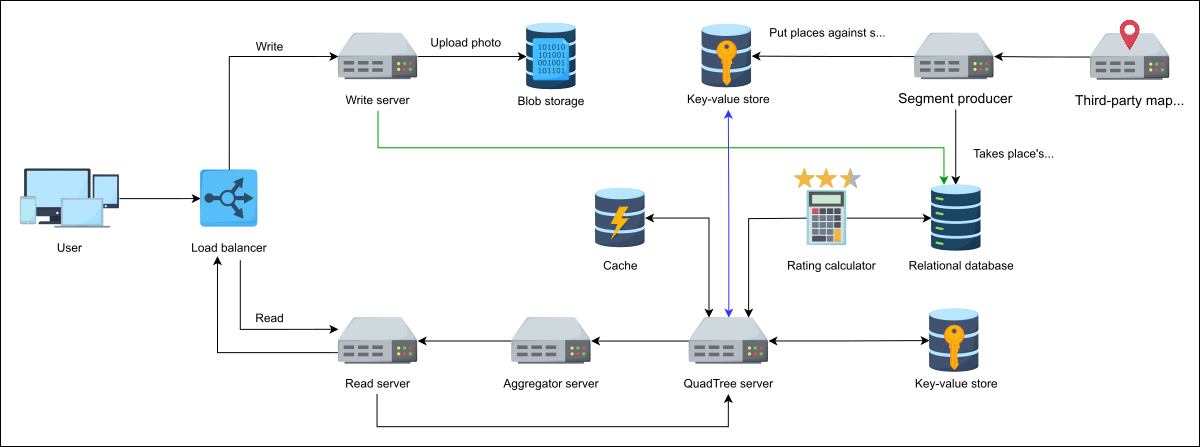
\includegraphics[width=0.5\textwidth]{Images/chapter_29/section_5518783229198336/5246501137022976.png}
 \caption{The updated detail design of Yelp}
\end{figure}

\subsection{Evaluation}\label{_RqRziRcG67MMRWoN4EUH}
\\
Let's see how our system design fulfills the non-functional requirements we identified in the initial lessons.

\subsubsection{Requirements compliance}\label{XkNq1G1trTzQgo3eIFsUx}

\begin{itemize}
\item
\protect\phantomsection\label{QibnD39uFfVphMRbAeTK9}
\textbf{Availability}: We partitioned the data into smaller segments instead of having to deal with a huge dataset consisting of all the places on the world map. This made our system highly available. We also replicated the QuadTrees data using key-value stores to ensure availability.
\item
\protect\phantomsection\label{w1pX73MragO7QSzo-YAD7}
\textbf{Scalability}: We split the whole world into smaller dynamic segments. This allows us to search for a place within a specific radius and shorten our search area. We then used QuadTrees in which each child node holds a single segment. Upon adding or removing a place, we can restructure our QuadTrees. So, we were able to make our system scalable.
\item
\protect\phantomsection\label{FKFzQ13xLnVoCa15PiE5h}
\textbf{Performance}: We reduced the latency by using caches. We cached all the famous and popular places, so request time was minimized.
\item
\protect\phantomsection\label{hyu2CtvkM3N4rknZuS-ME}
\textbf{Consistency}: The users have a consistent view of the data regarding places, reviews, and photos because we used reliable and fault-tolerant databases like key-value stores and relational databases.
\end{itemize}
\\
In the previous lesson, we chose a \textbf{SQL database} and a \textbf{key-value store} to design Yelp. How does replacing SQL with NoSQL impact the design? Discuss its impact on nonfunctional requirements like scalability and consistency. Also, discuss schema flexibility and the impact on the performance of complex queries.

\textbf{Question:}

How does replacing SQL with NoSQL impact the design?

\textbf{Reference Answer:}

SQL database: Yelp system will have different tables like ``Users,'' ``Place,'' ``Reviews,'' ``Photos,'' and others as described below. The data in these tables is inherently relational and structured. We need to perform queries like places a user visited, reviews they added, or view all the reviews of a specific place. It 's easy to perform such queries in a SQL-based database. We also want all users to have a consistent view of the data, and SQL-based databases are better suited for such use cases. We
'll use reliable and scalable databases, as is discussed in the Database building block.
\\
Key-value stores: We'll need to fetch the places in a segment efficiently. For that, we store the list of places against a segment ID in a key-value store to minimize searching time. We also save the QuadTree information in the key-value store, by storing the QuadTree data against a unique ID.
\\
NoSQL databases excel in scalability, allowing for horizontal scaling to handle large volumes of data and high traffic loads. However, they often prioritize availability and partition tolerance over strict consistency, leading to eventual consistency models that may result in temporary data inconsistencies. No SQL databases offer schema flexibility, enabling dynamic data models without predefined schemas, but they may struggle with complex queries compared to SQL databases, which excel in supporting complex data analysis and reporting. Ultimately
, the choice between SQL and NoSQL should consider the specific requirements of the application and the trade-offs between scalability, consistency, schema flexibility, and query performance.

\subsection{Summary}\label{e6L3XN3URCeSjwSeu98Dn}
\\
The proximity-based servers allow the user to search for a specific place or places nearby. The map data of the world is huge and dividing it into segments and finding the specific segment was a challenge in itself. So , we used QuadTrees to optimize our search and provided the user with a list of places with minimum latency.

% End of section content